\documentclass{beamer}
\usepackage[utf8]{inputenc}

\usetheme{Madrid}
\usecolortheme{default}
\usepackage{amsmath,amssymb,amsfonts,amsthm}
\usepackage{txfonts}
\usepackage{tkz-euclide}
\usepackage{listings}
\usepackage{adjustbox}
\usepackage{array}
\usepackage{tabularx}
\usepackage{gvv}
\usepackage{lmodern}
\usepackage{circuitikz}
\usepackage{tikz}
\usepackage{graphicx}

\setbeamertemplate{page number in head/foot}[totalframenumber]

\usepackage{tcolorbox}
\tcbuselibrary{minted,breakable,xparse,skins}



\definecolor{bg}{gray}{0.95}
\DeclareTCBListing{mintedbox}{O{}m!O{}}{%
  breakable=true,
  listing engine=minted,
  listing only,
  minted language=#2,
  minted style=default,
  minted options={%
    linenos,
    gobble=0,
    breaklines=true,
    breakafter=,,
    fontsize=\small,
    numbersep=8pt,
    #1},
  boxsep=0pt,
  left skip=0pt,
  right skip=0pt,
  left=25pt,
  right=0pt,
  top=3pt,
  bottom=3pt,
  arc=5pt,
  leftrule=0pt,
  rightrule=0pt,
  bottomrule=2pt,
  toprule=2pt,
  colback=bg,
  colframe=orange!70,
  enhanced,
  overlay={%
    \begin{tcbclipinterior}
    \fill[orange!20!white] (frame.south west) rectangle ([xshift=20pt]frame.north west);
    \end{tcbclipinterior}},
  #3,
}
\lstset{
    language=C,
    basicstyle=\ttfamily\small,
    keywordstyle=\color{blue},
    stringstyle=\color{orange},
    commentstyle=\color{green!60!black},
    numbers=left,
    numberstyle=\tiny\color{gray},
    breaklines=true,
    showstringspaces=false,
}
%------------------------------------------------------------
%This block of code defines the information to appear in the
%Title page
\title %optional
{4.3.34}
\date{September 15, 2025}
%\subtitle{A short story}

\author % (optional)
{Sai Hasini Pappula - EE25BTECH11044}



\begin{document}
\begin{frame}{Question}
\begin{block}{Problem}
If the line
\[
\frac{x}{a} + \frac{y}{b} = 1
\]
passes through the points $(2,-3)$ and $(4,-5)$, find $(a,b)$.
\end{block}
\end{frame}

% --- Frame 2: Matrix Formulation ---
\begin{frame}{Solution}
Substituting the points:
\begin{align}
\frac{2}{a} - \frac{3}{b} &= 1, \\
\frac{4}{a} - \frac{5}{b} &= 1.
\end{align}

Let
\begin{equation}
u = \frac{1}{a}, \quad v = \frac{1}{b}.
\end{equation}

Then the system becomes
\begin{equation}
\begin{bmatrix}
2 & -3 \\
4 & -5
\end{bmatrix}
\begin{bmatrix}
u \\ v
\end{bmatrix}
=
\begin{bmatrix}
1 \\ 1
\end{bmatrix}.
\end{equation}
\end{frame}

% --- Frame 3: Gauss-Jordan Elimination ---
\begin{frame}{Solution}
Start with the augmented matrix:
\[
\left[\begin{array}{cc|c}
2 & -3 & 1 \\
4 & -5 & 1
\end{array}\right]
\]

Row operations:
\begin{align}
R_2 &\to R_2 - 2R_1, \\
R_1 &\to R_1 + 3R_2, \\
R_1 &\to \tfrac{1}{2}R_1.
\end{align}

Final reduced form:
\[
\left[\begin{array}{cc|c}
1 & 0 & -1 \\
0 & 1 & -1
\end{array}\right]
\]
\end{frame}

% --- Frame 4: Final Answer ---
\begin{frame}{Final Answer}
Thus,
\begin{equation}
\begin{bmatrix} u \\ v \end{bmatrix}
= \begin{bmatrix} -1 \\ -1 \end{bmatrix}.
\end{equation}

Back-substitute:
\begin{align}
u &= \frac{1}{a} = -1 \;\Rightarrow\; a=-1, \\
v &= \frac{1}{b} = -1 \;\Rightarrow\; b=-1.
\end{align}

\begin{equation}
\boxed{(a,b) = (-1,-1)}
\end{equation}

Hence, the line is
\begin{equation}
x+y = -1.
\end{equation}
\end{frame}
% --- Frame 1: C Code (Part 1) ---
\begin{frame}[fragile]{C Code (Part 1)}
\begin{lstlisting}
#include <stdio.h>
int main() {
    // Augmented matrix for the system:
    // 2u - 3v = 1
    // 4u - 5v = 1
    double A[2][3] = {
        {2, -3, 1},
        {4, -5, 1}
    };
    // Step 1: R2 -> R2 - 2R1
    A[1][0] = A[1][0] - 2*A[0][0];
    A[1][1] = A[1][1] - 2*A[0][1];
    A[1][2] = A[1][2] - 2*A[0][2];
\end{lstlisting}
\end{frame}

% --- Frame 2: C Code (Part 2) ---
\begin{frame}[fragile]{C Code (Part 2)}
\begin{lstlisting}
    // Step 2: R1 -> R1 + 3R2
    A[0][0] = A[0][0] + 3*A[1][0];
    A[0][1] = A[0][1] + 3*A[1][1];
    A[0][2] = A[0][2] + 3*A[1][2];
    // Step 3: R1 -> R1 / 2
    A[0][0] /= 2;
    A[0][1] /= 2;
    A[0][2] /= 2;
    // Extract solution
    double u = A[0][2];
    double v = A[1][2];
    double a = 1.0 / u;
    double b = 1.0 / v;
    printf("u = %lf, v = %lf\n", u, v);
    printf("a = %lf, b = %lf\n", a, b);
    
    return 0;
}
\end{lstlisting}
\end{frame}


% ---------------- Python code 1 ----------------
\begin{frame}[fragile]{Python Code (Part 1)}
\lstset{language=Python}
\begin{lstlisting}
import ctypes
import numpy as np
import matplotlib.pyplot as plt

# Load the shared library
lib = ctypes.CDLL("code.so")

# Define the function signature for points
lib.points.argtypes = [
    ctypes.c_float,  # x_0
    ctypes.c_float,  # y_0
    ctypes.c_float,  # x_end
    ctypes.c_float,  # h
    np.ctypeslib.ndpointer(dtype=np.float32, ndim=1),  
    np.ctypeslib.ndpointer(dtype=np.float32, ndim=1),  
    ctypes.c_int     # steps
]
\end{lstlisting}
\end{frame}

% ---------------- Python code 2 ----------------
\begin{frame}[fragile]{Python Code (Part 2)}
\lstset{language=Python}
\begin{lstlisting}
# Parameters for simulation
x_0, y_0 = 0.0, 2.0
x_end, step_size = 1.0, 0.001
steps = int((x_end - x_0) / step_size) + 1

x_points = np.zeros(steps, dtype=np.float32)
y_points = np.zeros(steps, dtype=np.float32)

# Call the points function
lib.points(x_0, y_0, x_end, step_size, 
           x_points, y_points, steps)

# Theoretical solution (C = -2)
def theoretical_solution(x):
    return (-x + 4 - 2*np.exp(x))
\end{lstlisting}
\end{frame}

% ---------------- Python code 3 ----------------
\begin{frame}[fragile]{Python Code (Part 3)}
\lstset{language=Python}
\begin{lstlisting}
# Generate theory curve
x_theory = np.linspace(x_0, x_end, 1000)
y_theory = theoretical_solution(x_theory)

# Plot results
plt.plot(x_points, y_points, 'ro-', 
         markersize=2, linewidth=4, label="sim")
plt.plot(x_theory, y_theory, 'b-', 
         linewidth=2, label="theory")

plt.xlabel("x")
plt.ylabel("y")
plt.legend()
plt.grid(True, linestyle="--")
plt.show()
\end{lstlisting}
\end{frame}


% ---------------- Plot ----------------
\begin{frame}{Plot of the Line}
\begin{center}
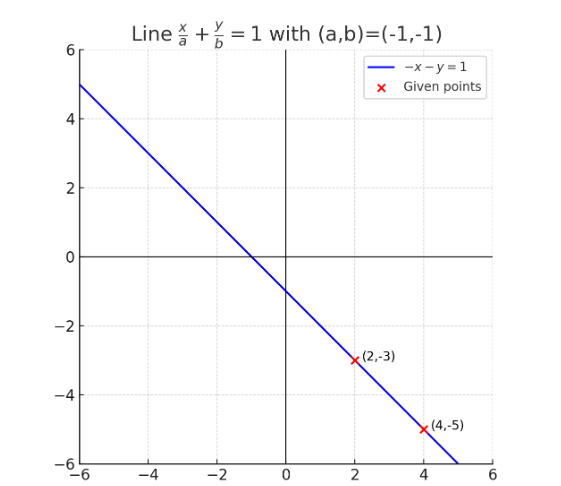
\includegraphics[width=0.7\columnwidth]{figs/plot6.png}
\end{center}
\end{frame}

\end{document}
